\documentclass{article}
\usepackage{soul}
\usepackage{xcolor}
\sethlcolor{pink}
\usepackage{amsmath}
\usepackage{amssymb}
\usepackage{cancel}
\usepackage{graphicx}
\usepackage{CJKutf8} 
\usepackage{tikz}

\usepackage{ulem}

\title{MATH1023/MATH1062 Calculas}
\author{Usyd Mingyuan Ba}
\date{\today}

\begin{document}

\maketitle

\section{Week1}
  \subsection{Differential Equation}
  \begin{enumerate}

    \item \textbf{Differential Equation(DE)}: A differential equation (DE) is a mathmatical equation that relates some \hl{function with its derivatives}

    \item \textbf{Order}: The order of a differential equation equals to a \hl{highest derivative} occuring in it.
      \begin{itemize}
        \item $\frac{dy}{dx} = -ky$ has order \hl{$1$}
        \item $\frac{dy}{dx} = y^{18} + \frac{d^5y}{dx^2}y + x^2$ has order \hl{5}
      \end{itemize}

    \item \textbf{Standard Form}: The standard form of a \hl{first-order differential equation} is
      \begin{center}
        $\frac{dy}{dx} = f(x,y)$
      \end{center}

    \item \textbf{General Solution}: A \hl{general solution} is a solution incoprating all constants of integration.

    \item \textbf{Initial Condition}: An initial condition is a pair $(x_0,y_0)$ such that $y(x_0) = y_0$


  \end{enumerate}


\section{Week2}
  \subsection{Direction Field}
  \begin{enumerate}
    \item \textbf{Definition}: A direction field of a DE
      \begin{center}
        $y' = f(x,y)$
      \end{center}
    consists of a grid of short line segments with slope $f(a,b)$ drawn at points $(a,b)$.So the line segment at $(a,b)$ is \hl{tangent} to any solution passing through $(a,b)$

    \item \textbf{Example}:Draw some solution curves on the given direction field for the DE:
      \begin{center}
        $y' = xy$
      \end{center}
    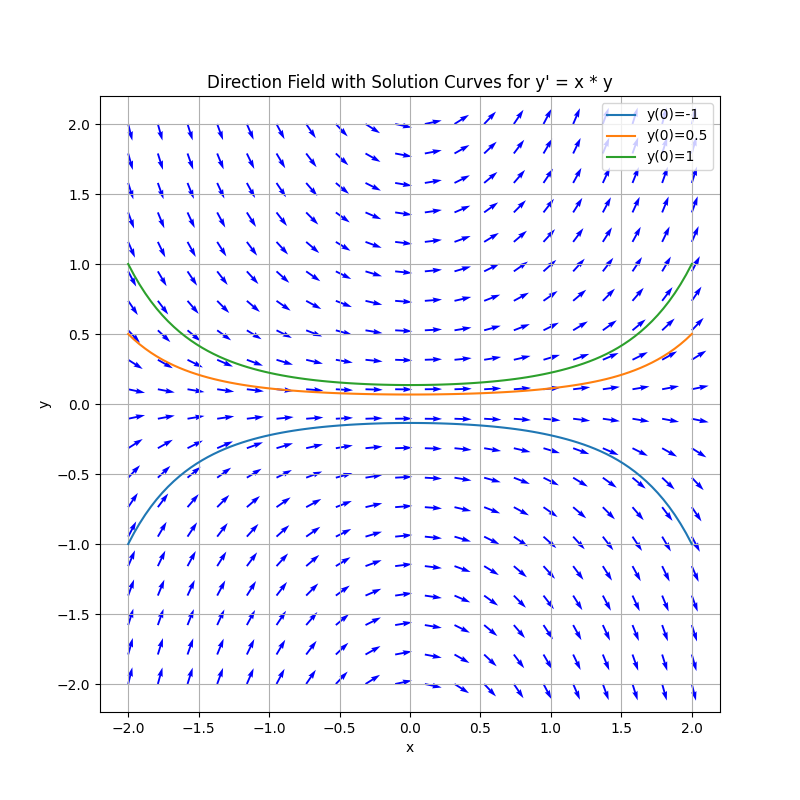
\includegraphics[width=\linewidth]{Graphs/direction_field.png}
  \end{enumerate}

  \subsection{Separable equations}

  \begin{enumerate}
    \item \textbf{Definition}: A first-order DE $y' = f(x,y)$ is called \hl{separable} if there are functions $g(x)$ and $h(y)$ such that \hl{$f(x,y) = g(x)h(y)$}, so a separable DE can be written
    \begin{center}
      \hl{$y' = g(x)h(y)$}
    \end{center}

    \item \textbf{Goal}: We want to find a method for solving separable DEs

    \item \textbf{Method}: We can solve a separable DE:
      \begin{center}
        $\frac{dy}{dx} = g(x)h(y)$
      \end{center}
    by separating variables.\\

    Dividing both sides by $h(y)$ gives 
      \begin{center}
        $\frac{1}{h(y)} \frac{dy}{dx} = g(x)$
      \end{center}

    Intergrating both sides gives:
      \begin{center}
        $\int \frac{1}{h(y)} = \int g(x) dx$ 
      \end{center}

    If we can find antiderivatives $H(y)$ for $\frac{1}{h(y)}$ and $G(x)$ for $g(x)$, then we have
      \begin{center}
        $H(y) = G(x) + C$ 
      \end{center}
  \end{enumerate}

  \section{Week3}
    \subsection{Modelling Population Growth}
      \begin{enumerate}
        \item \textbf{Constant Growth}: This occurs when the population $x$ increases at a constant rate. The DE is 
          \begin{center}
            $\frac{dx}{dt} = k$
          \end{center}
          where k is constant

        \item \textbf{Exponential Growth}: The exponential growth model assumes the growth rate is proportional to the size of the population.

        The general form of a DE modelling exponential growth is 
          \begin{center}
            $\frac{dx}{dt} = kx$
          \end{center}
          where k is constant

        \item \textbf{Logistic Growth}: Exponential growth is \hl{not} a realistic growth model for all values of $t$. \hl{A small animal population} with unlimited resources of food and space \hl{may show exponential growth initially}

        As the population gets larger there will be food shortages, overcrowding, and other factors that \hl{slow down the growth rate}.

        \hl{The growth rate k should decrease as the population x increases.}

        Since k is no longer constant, we write $k=g(x)$, so the DE becomes 
          \begin{center}
            $\frac{dx}{dt} = g(x)x$
          \end{center}

        A small population can growth exponentially, se we want \hl{$g(x) \approx k$} when \hl{$x \approx 0$}. But \hl{as x increases $g(x)$ should decrease.}

        The simplest formula with this behaviour is 
          \begin{center}
            $g(x) = k - ax$
          \end{center}

        So the DE becomes 
          \begin{center}
            $\frac{dx}{dt} = (k-ax)x$
          \end{center}

        We introduce a new constant $b = \frac{k}{a}$ so
          \begin{center}
            $(k-ax)x = ax (\frac{k}{a}-x) = ax(b-x)$
          \end{center}

        Let $\frac{b}{a} = b$, the logistic DE is then given by

          \begin{center}
            $\frac{dx}{dt} = ax(b-x)$
          \end{center}
      \end{enumerate}

  \section{week4}

    \subsection{First-order linear DEs}
      \begin{enumerate}
        \item \textbf{First-order linear differential equation}: A first-order linear differential equation is a DE of the form:
          \begin{center}
            $\frac{dy}{dx} + p(x) y = q(x)$
          \end{center}
          \textbf{$\frac{dy}{dx}$ and $y$ occur only linearly}

        \item \textbf{How to solve first-order linear DEs ?}: The idea is multiplying the DE by a function $r(x)$ give:
          \begin{center}
            $r(x) \frac{dy}{dx} + r(x)p(x) = r(x)q(x)$
          \end{center}

          If we can find $r(x)$ such that:
          \begin{center}
            $r(x) \frac{dy}{dx} + r(x)p(x) =$ \hl{$ \frac{d}{dx}(r(x)y(x))$}
          \end{center}

          then the DE becomes:
          \begin{center}
            \hl{$\frac{d}{dx}(r(x)y(x))$} $= r(x)q(x)$
          \end{center}

          Integrating with respect to x gives:
          \begin{center}
            $\int \frac{d}{dx}(r(x)y(x))dx = \int (r(x)q(x))dx$ \\
            $\rightarrow$ \\
            $r(x)y(x) = \int r(x)q(x)dx + C$

          \end{center}

          so the general solution is

          \begin{center}
            $y = \frac{1}{r(x)} [\int r(x)q(x) dx + C]$
          \end{center}

        \item \textbf{Integrating factor}: The function
          \begin{center}
            $r(x) = e^{\int p(x) dx}$
          \end{center}
          is an intergrating factor for the first-order linear DE

          \begin{center}
            $\frac{dy}{dx} + p(x)y = q(x)$
          \end{center}

        \item \textbf{General Solution } the general solution of the DE is 
          \begin{center}
            $y = \frac{1}{r(x)} [\int r(x)q(x) dx + C]$
          \end{center}

      \end{enumerate}


  \section{week5}

    \subsection{Higher order differential equations}

      Higher order DEs involve higher order derivatives.For example, the DE:

      \begin{center}
        $\frac{d^2 y}{dx^2} + f(x,y) \frac{dy}{dx} = g(x,y)$
      \end{center}
      is a \hl{second-order differential} equation.

      \begin{enumerate}
        \item Solving higher-order DEs is harder.
        \item The general solution of a second-order DE has 2 degrees of freedom, so needs two initial conditions.
        \item The general solution of an \hl{nth-order DE has n degrees of freedom}, so \hl{needs n initial conditions}.
      \end{enumerate}

    \subsection{Second-order linear DEs with constant coefficients}
      \begin{enumerate}
        \item \textbf{Definition} A \hl{second-order linear differential equation} is a DE that can be expressed in the form:
        \begin{center}
          $\frac{d^2y}{dx} + f_1(x)\frac{dy}{dx} + f_0(x)y = g(x)$
        \end{center}

        \hl{The DE is linear in $y$ and its derivatives.}

        \item \textbf{homogeneous/inhomogeneous}
            \begin{itemize}
              \item The DE is homogeneous if $g(x) = 0$
              \item The DE is inhomogeneous if $g(x) \neq 0$
            \end{itemize}

        If \hl{$g(x) = 0,f_0(x) = a, f_1(x) = b$ for $a,b \in \mathbb{R}$}, then we have a \hl{homogeneous second-order linear differential equation} with constant coefficient:

        \begin{center}
          $\frac{d^2 y}{dx^2} + a \frac{dy}{dx} + by = 0$
        \end{center}

        \item Solve the above DE : 
        \begin{center}
          $\frac{d^2 y}{dx^2} + a \frac{dy}{dx} + by = 0$
        \end{center}

        
        \begin{itemize}
          \item \textbf{Observation 1}: y is a linear combination of its first two derivatives, so we try:
          \begin{center}
            $y(x) = e^{mx}$
          \end{center} 

          We have

          \begin{center}
            $\frac{dy}{dx} = me^{mx}, \frac{d^2y}{dx^2} = m^2e^{mx}$
          \end{center} 

          \item \textbf{Observation 2}: Find m such that $y = Ce^{mx}$ satisfies the DE
          \begin{center}
            $\frac{d^2y}{dx^2} + a\frac{dy}{dx} + by = 0$
          \end{center}
          substituting y and its derivatives we get:
          \begin{center}
            $Cm^2e^{mx} + aCme^{mx} + bCe^{mx} = 0$\\
            $\Rightarrow Ce^{mx}(m^2+am+ b) = 0$\\
            $\Rightarrow m = \frac{-a \pm \sqrt{a^2 - ab}}{2} $
          \end{center}

          So we have  2 solutions

          \begin{center}
            $m_1 = \frac{-a + \sqrt{a^2 - ab}}{2}, m_2 = \frac{-a - \sqrt{a^2 - ab}}{2}$
          \end{center}       

          \item \textbf{Observation 3:} Show that if $m = m_1,m_2$ are solutions of $m^2 + am +b$,then \hl{$y = C_1e^{m_1x} + C_2e^{m_2x}$}, satisfies the DE

          \begin{center}
            $\frac{d^2y}{dx^2} + a\frac{dy}{dx} + by = 0$
          \end{center}

          we have 
          \begin{center}
            $y = C_1e^{m_1x} + C_2e^{m_2x}$\\
            $\Rightarrow \frac{dy}{dx} = m_1C_1e^{m_1x} + m_2C_2e^{m_2x}$\\
            $\Rightarrow \frac{d^2y}{dx^2} = m_1^2C_1e^{m_1x} + m_2^2C_2e^{m_2x}$
          \end{center}

          substituting into the DE we get

          \begin{center}
            $2$\\
            $\Rightarrow \frac{dy}{dx} = m_1C_1e^{m_1x} + m_2C_2e^{m_2x}$\\
            $\Rightarrow \frac{d^2y}{dx^2} = m_1^2C_1e^{m_1x} + m_2^2C_2e^{m_2x}$
          \end{center}

          substituting into the DE we get 

          \begin{align*}
            \frac{d^2 y}{dx^2} + a \frac{dy}{dx} + by &= m_1^2 C_1 e^{m_1 x} + m_2^2 C_2 e^{m_2 x} + a \left( m_1 C_1 e^{m_1 x} + m_2 C_2 e^{m_2 x} \right) + b \left( C_1 e^{m_1 x} + C_2 e^{m_2 x} \right) \\
            &= C_1 e^{m_1 x} \left( m_1^2 + a m_1 + b \right) + C_2 e^{m_2 x} \left( m_2^2 + a m_2 + b \right) \\
            &= 0
          \end{align*}


          \item \textbf{formal solution:} 
            We now have a good candidate for a general solution of the DE:
            \begin{center}
              $y =C_1e^{m_1x} + C_2e^{m_2x}$ 
            \end{center}
            Where $m_1 = \frac{-a + \sqrt{a^2-4b}}{2}$,$m_2 = \frac{-a - \sqrt{a^2-4b}}{2}$ are solutions of $m^2 + am +b = 0$. We have 3 cases to consider:



            \begin{itemize}
                \item \textbf{Case 1}: For \hl{$a^2 > 4b$} we have 2 distinct real solutions
                \begin{center}
                  $m_1 \neq m_2, m_1,m_2 \in \mathbb{R}$
                \end{center}
                The general solution is 
                \begin{center}
                  $y =C_1e^{m_1x} + C_2e^{m_2x}$
                \end{center}


                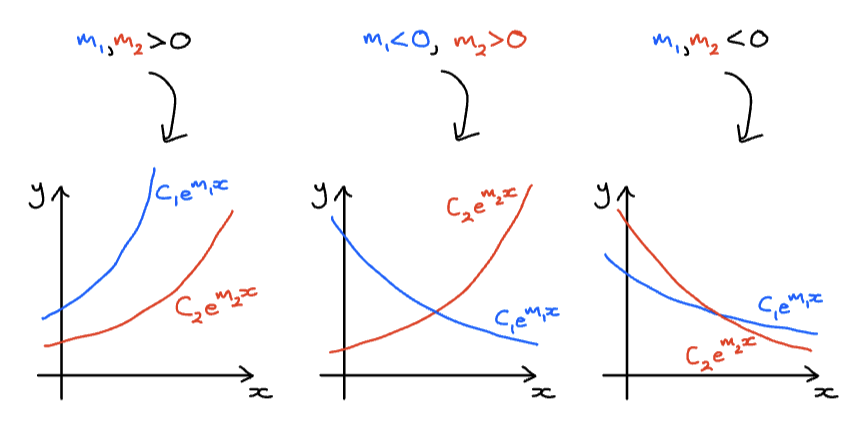
\includegraphics[width=\linewidth]{Graphs/w5_1.png}


                \item \textbf{Case 2}: For \hl{$a^2 < 4b$} we have 2 distinct complex solutions:
                \begin{center}
                  $m_1,m_2 = \frac{-a \pm \sqrt{a^2-4b}}{2} = \frac{-a \pm 2ik}{2} = - \frac{a}{2} \pm ik$\\
                  where \hl{$k = \frac{1}{2} \sqrt{4b-a^2} > 0$}
                \end{center}
                Using Euler's formula:
                \begin{center}
                  $e^{ikx} = cos(kx) + isin(kx)$
                \end{center}
                
                We have

                \[
                y = C_1 e^{m_1 x} + C_2 e^{m_2 x}
                \]

                \[
                = C_1 e^{\left(-\frac{a}{2} + ik\right)x} + C_2 e^{\left(-\frac{a}{2} - ik\right)x}
                \]

                \[
                = e^{-\frac{a}{2}x} \left( C_1 e^{ikx} + C_2 e^{-ikx} \right)
                \]

                \[
                = e^{-\frac{a}{2}x} \left( C_1 \left(\cos(kx) + i\sin(kx)\right) + C_2 \left(\cos(kx) - i\sin(kx)\right) \right)
                \]

                \[
                = e^{-\frac{a}{2}x} \left( \left(C_1 + C_2\right) \cos(kx) + i \left(C_1 - C_2\right) \sin(kx) \right)
                \]

                \[
                = e^{-\frac{a}{2}x} \left( D_1 \cos(kx) + D_2 \sin(kx) \right)
                \]

                So the general solution is:
                \hl{$y = e^{-\frac{a}{2}x} \left( D_1 \cos(kx) + D_2 \sin(kx) \right)$}

                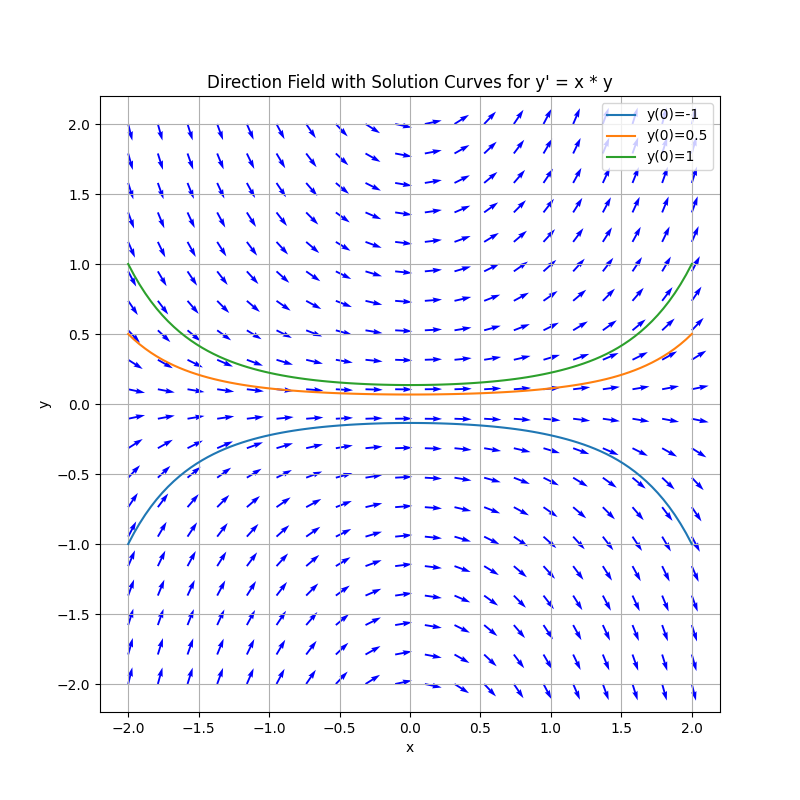
\includegraphics[width=\linewidth]{Graphs/direction_field.png}


                \item \textbf{Case 3}: For $a^2 = 4b$ we have 1 real solution:
                  \begin{center}
                    \( m_1 = m_2 = \frac{-a \pm \sqrt{a^2 - 4b}}{2} = -\frac{a}{2} \)
                  \end{center}
                  Our solution becomes

                  \[
                  y = C_1 e^{-\frac{a}{2}x} + C_2 e^{-\frac{a}{2}x}
                  \]

                  \[
                  = \left( C_1 + C_2 \right) e^{-\frac{a}{2}x}
                  \]

                  \[
                  = D e^{-\frac{a}{2}x}
                  \]

                  Here, \( D \) is a constant (\( D = C_1 + C_2 \)), which means we only have \hl{1 degree of freedom, so this is not a general solution}.

                  \newpage

                  We look for a general solution of the form
                  \begin{center}
                    $y = f(x)e^{-\frac{a}{2}x}$
                  \end{center}

                  Substituting \( y \) and its derivatives into the differential equation (DE)

                  \[
                  \frac{d^2y}{dx^2} + a\frac{dy}{dx} + by = 0
                  \]

                  gives

                  \[
                  e^{-\frac{a}{2}x} \left( f''(x) + \frac{1}{4}(4b - a^2)f(x) \right) = 0 \quad \text{(exercise)}
                  \]

                  Since \( e^{-\frac{a}{2}x} \neq 0 \),

                  \[
                  f''(x) = \frac{1}{4}(a^2 - 4b)f(x) = 0
                  \]

                  which implies

                  \[
                  f'(x) = C_2
                  \]

                  \[
                  f(x) = C_2 x + C_1
                  \]

                  Hence, the general solution is

                  \[
                  y = (C_1 + C_2 x) e^{-\frac{a}{2}x}
                  \]


            \end{itemize}
        \end{itemize}

      \end{enumerate}

  \newpage

  \section{week6}
    % \begin{CJK}{UTF8}{gbsn} % 开始中文环境,gbsn是简体中文宋体
    % 你好,世界! % 在这里可以输入中文
    % \end{CJK}
    \subsection*{Simple harmonic motion}
    \begin{itemize}
      \item Periodic bhaviour \hl{without} damping is modelled by the DE
        \begin{center}
        $\frac{d^2x}{dt^2} + bx = 0,b>0$\\
        or\\
        $\ddot{x} + w_{0}^2x = 0$
        \end{center}

      \item We can express the solution as 
        \begin{center}
          $x = Acos(w_0t + \phi)$
        \end{center}
        \begin{itemize}
          \item $A$ = amplitude
          \item $w_0$ = frequency
          \item $\phi$ =  phase
          \item $T = \frac{2 \pi}{w_0}$ = period
        \end{itemize}
    \end{itemize}

    \subsection*{Damped harmonic oscillator}
    \begin{itemize}
      \item Periodic behaviour \hl{with} damping is  modelled by the DE:
        \begin{center}
          $\frac{d^2x}{dt^2} + a \frac{dx}{dt} + bx = 0$
        \end{center}

        with $a = 2 \gamma$,$b = \omega_0^2$, or
        \begin{center}
          $\ddot{x} + 2 \gamma \dot{x} + \omega_0^{2}x = 0$
        \end{center}

      \item The characteristic equation is 
        \begin{center}
          $m^2 + am + b = 0$
        \end{center}
        which has solution 
        \begin{center}
          $ m = \frac{-a \pm \sqrt{a^2 - 4b}}{2} = - \gamma \pm \sqrt{\gamma^2 - \omega_0^2}$
        \end{center}

    \end{itemize}

    \subsection*{Inhomogeneous second-order linear DEs with constant coefficients}

    \begin{itemize}
      \item An \hl{inhomogeneous scond-order linear differential equation} with constant coefficients is a DE that can be expressed in the form:
      \begin{center}
        $\frac{d^2y}{dx^2} + a\frac{dy}{dx} + by = g(x)$
      \end{center}

      \item \textbf{theorem}: Let $y_p(x)$ be a particular solution of an \hl{inhomogeneous linear DE} and let $y_h(x)$ be the \hl{general solution} of the corresponding homogeneous DE. Then the general solution of the inhomogeneous DE is the
      \begin{center}
        $y(x) = y_h(x) + y_p(x)$
      \end{center}

      \item \hl{systems of first-order linear DEs with constant coefficients}: A system of two first-order DEs with constant coefficients has the form:

      \begin{center}
        $\frac{dx}{dt} = ax + by$ \texttt{(*)},\\
        $\frac{dy}{dt} = cx + fy$ \texttt{(**)}
      \end{center}

      to solve this system, we follow the following steps:
      \begin{enumerate}
        \item Differentiate \texttt{(*)}
          \begin{center}
            $\frac{d^2x}{dt^2} = a\frac{dx}{dt} +$ \hl{$b \frac{dy}{dt}$} \texttt{(I)}
          \end{center}

        \item Substitude the right hand side of of \texttt{(**)} into \texttt{(I)}
          \begin{center}
            $\frac{d^2x}{dt^2} = a\frac{dx}{dt} +$ \hl{$b(cx + fy)$} \texttt{(II)}
          \end{center}

        \item Rearrange \texttt{(*)} to make y the subject
          \begin{center}
            $y = \frac{1}{b} (\frac{dx}{dt} - ax)$ \texttt{(III)}
          \end{center} 
        \item Substitude the right hand side of \texttt{(III)} into \texttt{(II)} 
          \begin{center}
            $\frac{d^2x}{dt^2} = a \frac{dx}{dt} + b(cx + 
            \frac{f}{b}(\frac{dx}{dt}-ax)) \rightarrow \frac{d^2x}{dt^2} = (a+f)\frac{dx}{dt} + (bx - af)x$
          \end{center}

        \item Solve the DE   
          \begin{center}
            $\frac{d^2x}{dt^2} - (a+f)\frac{dx}{dt} - (bc-af)x = 0$ for x.
          \end{center}
        \item Substitute x into \texttt{(**)} and solve the \hl{first-order linear DE} for y
        \begin{center}
          $\frac{dy}{dt} = cx + fy \rightarrow \frac{dy}{dt} + p(t)y = q(t)$

        \end{center}       
      \end{enumerate}
    \end{itemize}

\section{Week7}
  \subsection*{2-dimensional plane}
    \begin{itemize}
      \item The \textbf{2-dimensional plane}, often called the $(x,y)$-plane, can be represented by the set
      \[
        \mathbb{R}^2 = \{(x,y) \mid x,y \in \mathbb{R}\}
      \]
      \item The \textbf{graph} of a function
      \[
        f: D \rightarrow \mathbb{R}, \quad y = f(x), \quad D \subseteq \mathbb{R}
      \]
      is given by the set
      \[
        \{(x,y) \in \mathbb{R}^2 \mid y = f(x), x \in D\}
      \]
      \item Curves in the plane can also be given by parametric equations:
      \[
        x = f(t), \quad y = g(t)
      \]
      where \( t \) is a parameter.
    \end{itemize}

  \subsection*{3-dimensional space}
    \begin{itemize}
      \item \textbf{3-dimensional space} can be represented by the set
      \[
        \mathbb{R}^3 = \{(x,y,z) \mid x,y,z \in \mathbb{R}\}
      \]
      \item \textbf{Right-handed system}: The \( x, y, z \) axes are a right-handed system. The positive \( x, y, z \) directions are determined by the right-hand rule:
        \begin{enumerate}
          \item Point the fingers of your right hand in the positive \( x \)-direction.
          \item Curl your fingers in the positive \( y \)-direction.
          \item Your thumb points in the positive \( z \)-direction.
        \end{enumerate}
    \end{itemize}

  \subsection*{Curves in $\mathbb{R}^3$}
    \begin{itemize}
      \item Curves in \( \mathbb{R}^3 \) can be represented using parametric equations:
      \[
        x = f(t), \quad y = g(t), \quad z = h(t)
      \]
      
      \item There is \hl{no} way of turning these parametric equations of a curve in space intoa single Cartesion equation
    \end{itemize}


  \subsection*{Surfaces in $\mathbb{R}^3$}
  \begin{itemize}
    \item A \textbf{surface} in $\mathbb{R}^3$ is given by a single equation involving $x,y,x$
    \item The general form of a plane is $ax + by + cz = d$
    \item The general form of a \textbf{sphere} with radius $r$ and centre $(a,b,c)$ is $(x-a)^2 (y-b)^2 + (z-c)^2 = r^2$
    \item The general form of a \textbf{paraboloid} is given by 
    \begin{center}
      $z = c \pm ((x-a)^2 + (y-b)^2)$
    \end{center}
  \end{itemize}

\section{Week8}
  \subsection*{Function of one variable}
  \begin{itemize}
  	\item \textbf{Definition}: Recall that a \hl{function of one real variable}
  		\begin{center}
  			$f: D \rightarrow \mathbb{R}, D \subseteq \mathbb{R}$
  		\end{center}
  		is a rule that assigns to each number $x \in D$ a number $f(x) \in \mathbb{R}$
  	\item The \textbf{domain} of $f$ is the \hl{set D of allowed inpus}.
  	\item The \textbf{natural domain} of $f$ is \hl{the largest subset of R of allowed inputs}.
  \end{itemize}

  \subsection*{Function of 2 variables}
  \begin{itemize}
  	\item \textbf{Definition:} A \hl{function of 2 real variables}:
  	\begin{center}
  		$f: D \rightarrow \mathbb{R}, D \subseteq \mathbb{R}^2$
  	\end{center}
  	is a \hl{rule that assigns to each pair $(x,y) \in D$ a number $f(x,y) \in \mathbb{R}$}

  	\item The \textbf{domain} of f is the \hl{set D of allowed inpus}

  	\item The \textbf{natrual domian of $f$} is the \hl{largest subset of $\mathbb{R}^2$ of allowed inputs}
  \end{itemize}

  \subsection*{Graphs of functions}
  \begin{itemize}
  	\item The \hl{graph} of a function of 2 variables:
  		\begin{center}
  			$f: D \rightarrow \mathbb{R}$
  		\end{center}
  		is the set of points
  		\begin{center}
  			$\{(x,y,f(x,y))\in \mathbb{R}^3 | (x,y) \in D\}$
  		\end{center}
		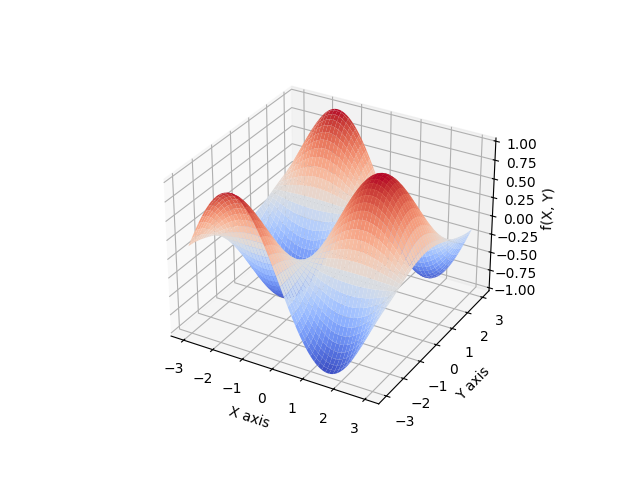
\includegraphics[width=1.0\textwidth, height=8cm]{Graphs/w8_1.png}

	\item We \hl{can not} get a full sphere as a function. It fails the vertical line test.
  \end{itemize}

  \subsection*{Level Curves}
  \begin{itemize}
  	\item \textbf{Definition:} A \hl{level cureve} of a function $f(x,y)$ is a curve in $\mathbb{R}^2$ defined by 
  	\begin{center}
  		$f(x,y) = c$
  	\end{center}
  	for a constant $c \in \mathbb{R}$

  	\item The level curves $f(x,y) = c$ are the intersections of the surface $z = f(x,y)$ with the planes $z=c$

	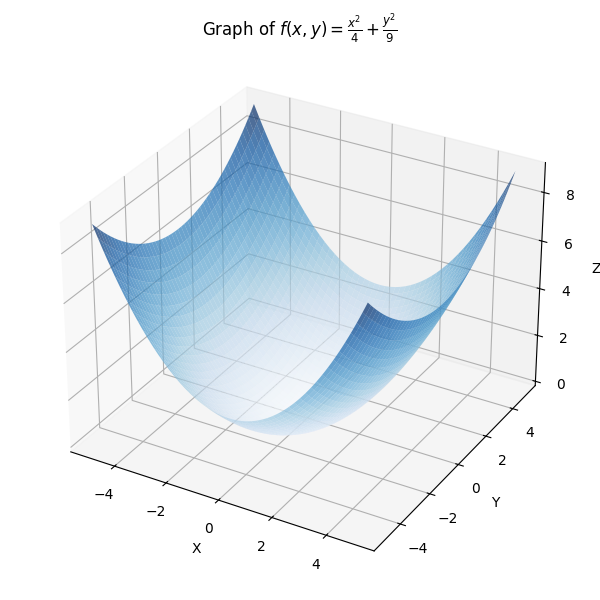
\includegraphics[width=\linewidth, height=6cm]{Graphs/w8_2.png}

	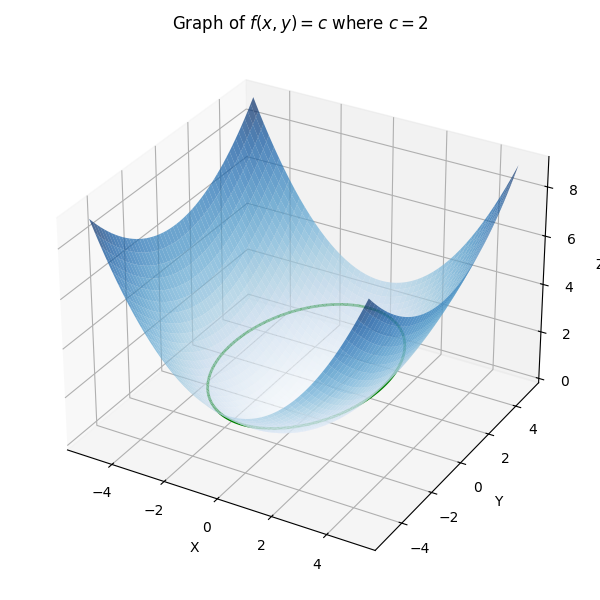
\includegraphics[width=\linewidth, height=6cm]{Graphs/w8_3.png}

	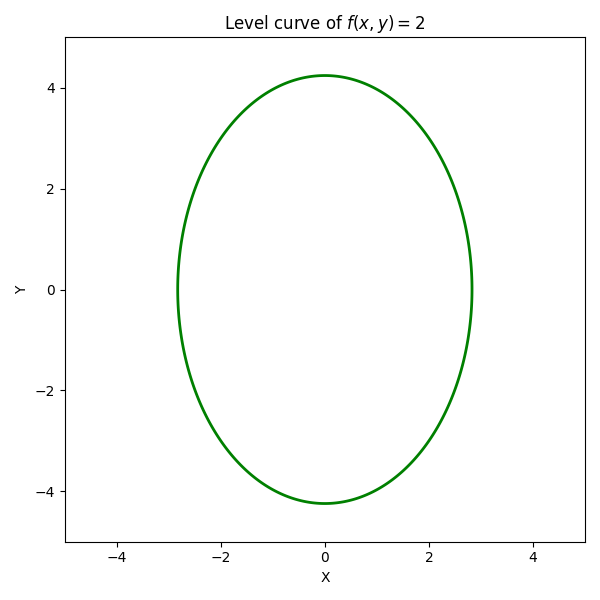
\includegraphics[width=\linewidth, height=6cm]{Graphs/w8_4.png}
  \end{itemize}

  \subsection*{Partial derivatives}
  \begin{itemize}
  	\item \textbf{Definition:} for a sufficiently smooth function of 2 variables
  	\begin{center}
  		$f: D \rightarrow \mathbb{R}, D \subseteq \mathbb{R}^2$
  	\end{center}
  	The \hl{partial derivative of $f$ with respect to $x$ at $(x,y) = (a,b)$ is:}
  	\begin{center}
  		$f_x(a, b) = \frac{\partial f}{\partial x}\Bigg|_{(x,y)=(a,b)} = \lim_{h \to 0} \frac{f(a+h,b) - f(a,b)}{h}$
  	\end{center}
  	and the \hl{partial derivative of $f$ with respect to $y$ at $(x,y) = (a,b)$} is 
  	\begin{center}
  		$f_x(a, b) = \frac{\partial f}{\partial y}\Bigg|_{(x,y)=(a,b)} = \lim_{h \to 0} \frac{f(a,b+h) - f(a,b)}{h}$
  	\end{center}

  	\item \textbf{Terminology}: If $f_x(a,b) = \frac{\partial f}{\partial x}\Bigg|_{(a,b)}$ exists \hl{for all $(a,b) \in D$}, then we say that $f$ \hl{is diffrentiable with respect to $x$ on D} and we write
  	\begin{center}
  		$f_x(x,y) = \frac{\partial f}{\partial x}(x,y)$
  	\end{center}
  	for the \hl{derivative function of f w.r.t. x.}

  	\item Similarly, If $f_y(a,b) = \frac{\partial f}{\partial y}\Bigg|_{(a,b)}$ exists \hl{for all $(a,b) \in D$}, then we say that $f$ \hl{is diffrentiable with respect to $y$ on D} and we write
  	\begin{center}
  		$f_y(x,y) = \frac{\partial f}{\partial y}(x,y)$
  	\end{center}
  	for the \hl{derivative function of f w.r.t. y.}

  	\item What do partial derivatives measure? For a sufficiently smooth function:
  	\begin{center}
  		$f: D \rightarrow \mathbb{R}, D \subset \mathbb{R}$
  	\end{center}
  	the partial derivatives $f_x = \frac{\partial f}{\partial x}$ measure the rate of change of $f$ on the $x$ direction. 

	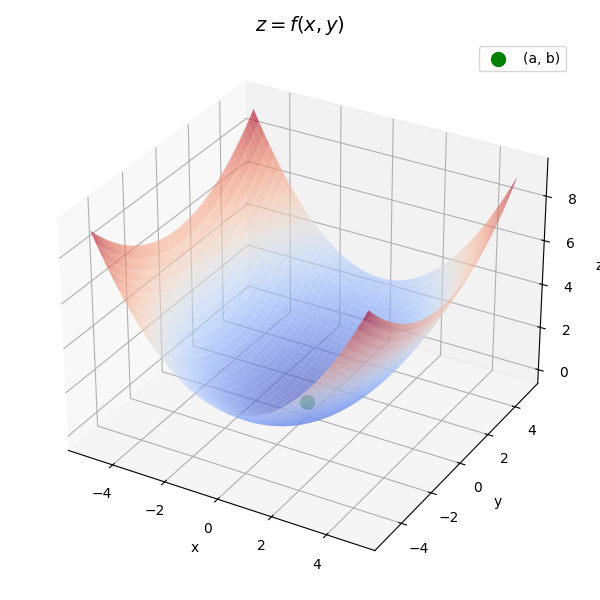
\includegraphics[width=\linewidth, height=6cm]{Graphs/w8_5.png}


	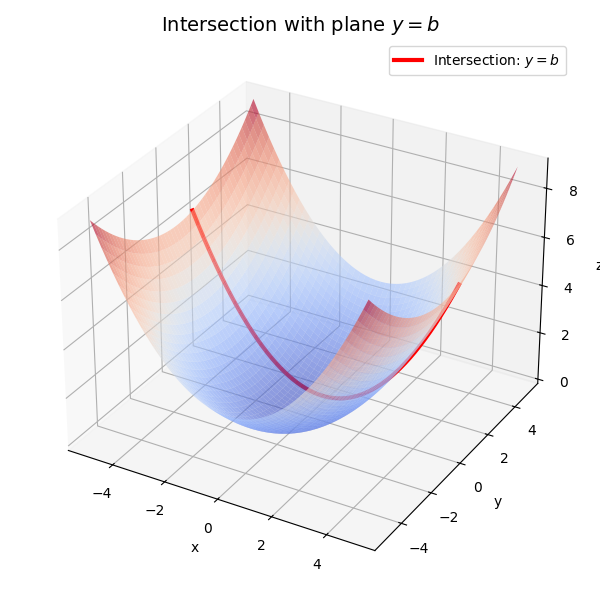
\includegraphics[width=\linewidth, height=6cm]{Graphs/w8_6.png}

	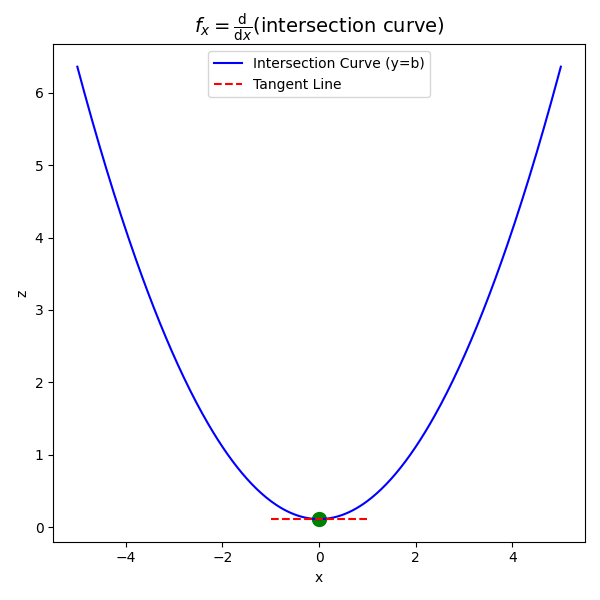
\includegraphics[width=\linewidth, height=6cm]{Graphs/w8_7.png}

	\item Here we have \hl{the intersection of the surface $z=f(x,y)$ and the plane $y=b$} is the function of one variable given by 
	\begin{center}
		$g(x) = f(x,b)$
	\end{center}
	The \hl{gradient} of the tangent to this curve at $x=a$ is given by
	\begin{center}
		$g'(a) = \lim_{h \to 0} \frac{g(a+h) - g(a)}{h}$ \\
		$= \lim_{h \to 0} \frac{f(a+h, b) - f(a, b)}{h}$ \\
		$= f_x(a, b)$
	\end{center} 

	\item How do we calculate partial derivatives?

	\begin{itemize}
		\item To calculate $f_x = \frac{\partial f}{\partial x}$
		\begin{enumerate}
			\item Imagine $y$ is a constant
			\item Differentiate as a function of one variable $x$.
		\end{enumerate}

		\item To calculate $f_y = \frac{\partial f}{\partial y}$
		\begin{enumerate}
			\item Imagine $x$ is a constant
			\item Differentiate as a function of one variable $y$.
		\end{enumerate}
	\end{itemize}

  \end{itemize}

  \subsection*{Tangent lines and plane}
  \begin{itemize}
    \item \textbf{tangent lines}: Given a differentiable function of 1 variable, we can consider the tangent line at $x = a$.

    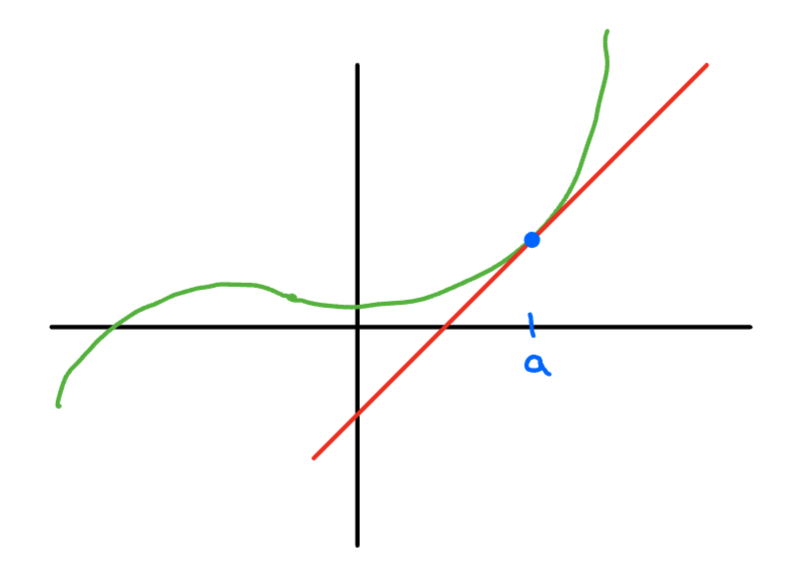
\includegraphics[width=\linewidth]{Graphs/w9_1.png}

    The equation of the tangent line is:
    $$
      y =f(a)+ f'(a)(x-a)
    $$

    \hl{The tangent is the best linear approximation to $f$ near $x = a$}


    \item \textbf{Tangent plane:} Consider the tangent plane at a point $(a,b)$ of a "nice" function of two variables
    $$
      f: D\rightarrow \mathbb{R}, D \subseteq \mathbb{R}^2
    $$

    The tangent plane is the best linear approximation to $f$ near $(x,y) = (a,b)$. It should have the same first-order partial derivatives.

    The equation of the tangent plane to $f$ at $(a,b)$ is
    $$
      z = f(a,b) +f_x(a,b)(x-a) + f_y(a,b)(y-b)
    $$

  \end{itemize}

  \section{Week 9}
  \subsection*{Approximating values of functions using tangents}
  \begin{itemize}
    \item \textbf{Differential:} The differential of a differentiable function $y = f(x)$ is 
    $$
      dy = f'(x)dx
    $$

    In Leibniz notation $dy = \frac{dy}{dx}dx$

    \item \textbf{Differential:} The differential of a differentiable function $z = f(x,y)$ is 
    $$
    dz = f_x(x,y)dx + f_y(x,y)dy
    $$

    \item \textbf{Approximation:} If $(x,y)$ is near $(a,b)$ then we have
    \begin{center}
      $ f(x,y) \approx f(a,b) + dz $\\
      $= f(a,b) + f_x(a,b)(x-a) +f_y(a,b)(y-b)$\\
      = z value of equation of tangent plane
    \end{center}
  \end{itemize}

  \subsection*{The total derivative}
  \begin{itemize}
    \item \textbf{Definition:} If $z = f(x,y), x = g(t),y = h(t)$ are differentiable functions, then the total derivative of z with respect to $t$ at $t = a$ is:
    $$
      \frac{dz}{dt} = \lim_{k \to 0} \frac{f(g(a+k), h(a+k)) - f(g(a), h(a))}{k}
    $$

    \item To calculate the total derivative, we user the total derivative rule:
    $$
      \frac{dz}{dt} = \frac{\partial z}{\partial x} \frac{dx}{dt} + \frac{\partial z}{\partial y} \frac{dy}{dt}
    $$

    \item \textbf{Chain Rule}: If $z = f(x,y),x=g(s,t),y = h(s,t)$ are differentiable functions, we have:
    $$
      \frac{\partial z}{\partial s} = \frac{\partial z}{\partial x} \frac{\partial x}{\partial s} + \frac{\partial z}{\partial y} \frac{\partial y}{\partial s}
    $$
    $$
      \frac{\partial z}{\partial t} = \frac{\partial z}{\partial x} \frac{\partial x}{\partial t} + \frac{\partial z}{\partial y} \frac{\partial y}{\partial t}
    $$
  \end{itemize}

  \subsection*{Implicit Differentiation}
  \begin{itemize}
    \item \textbf{Implicit function theorem:(IFT):} Let $C \subseteq \mathbb{R}^2$ be a curve defined by $f(x,y) = k$ for some differentiable function $f: D \rightarrow \mathbb{R}, D \subseteq \mathbb{R}^2$ and $k \in \mathbb{R}$.\\
    If $(a,b) \in D, f(a,b) = k$ and $f_y(a.b) \neq 0$ then C can be described around $(a,b)$ by a function
    $$
      y = g(x)
    $$

    \item \textbf{Application of the IFT:} If we can apply the IFT then we can find $\frac{dy}{dx}$ using the following method:
      \begin{enumerate}
        \item Start with $f(x,y) = k$
        \item Use the IFT to express $y$ locally as a function of $x$ and substitute into the formula for the curve
        $$
          f(x,g(x)) = k
        $$
        \item Use the chain rule to differentiate with respect to x
        $$
          f_x\frac{dx}{dx} + f_y\frac{dg}{dx} = 0
        $$
        \item Solve for $\frac{dg}{dx}$
        $$
          \frac{dg}{dx} = -\frac{fx}{fy}
        $$
      \end{enumerate}

      \item \textbf{A formula for $\frac{dy}{dx}$}:
        $$
          \left. \frac{dy}{dx} \right|_{x=a} = - \frac{f_x(a, b)}{f_y(a, b)}
        $$
  \end{itemize}

  \section*{Week 10+11}
  \newcommand{\unitv}[1]{\hat{\underset{\sim}{#1}}}
  \newcommand{\vect}[1]{\underset{\sim}{#1}}
  \newcommand{\DEF}{\textbf{Definition:\ }}
  \newcommand{\len}[1]{||#1||}

  \subsection*{Directional derivatives}
  \begin{itemize}
  	\item \DEF Let $\vect{u}$ be a nonzero vector with $\unitv{u} = u_1 \vect{i} + u_2 \vect{j}$, and let $f(x,y)$ be a differentiable function. The \hl{directional derivative} of $f$ at $(a,b)$ in the direction of $\vect{u}$ is:
  	\[
	\left( D_{\unitv{u}} f \right)(a, b) = \lim_{h \to 0} \frac{f(a + u_1 h, b + u_2 h) - f(a, b)}{h}
	\]

	\item Remarks
	\begin{itemize}
		\item $(D_{\vect{i} })(a,b) = f_x(a,b)$
		\item $(D_{\vect{j} })(a,b) = f_y(a,b)$
	\end{itemize}

	\item If $f(x,y)$ is differentiable, and $\unitv{u} = u_1\vect{i} + u_2\vect{j}$ is a unit vector, then
	$$
	D_{\unitv{u}}f (a, b) = f_x(a,b)u_1 + f_y(a,b)u_2
	$$

	\item How to compute $D_{\vect{u}}f$\ (Method 1)
		\begin{enumerate}
			\item Find the unit vector in the direction
			\item Find the first-order partial derivatives at the point
			\item Apply the above formula
		\end{enumerate}
  \end{itemize}

  \subsection*{Gradient Vector}
  \begin{itemize}
  	\item \DEF Suppose we haves a differentiable function :
  	$$
  	 f: D \rightarrow R, D \subseteq R^2
  	$$

  	The \hl{gradient of f} is the vecotr valued function :
  	$$
  		\nabla f : D \rightarrow R^2
  	$$
  	defined by
  	$$
  		\nabla f(x,y) = f_x(x,y)\vect{i} + f_y(x,y)\vect{j}
  	$$

  	\item How to compute $D_{\vect{u}}f$ (Method 2):
  	$$
  		D_{\vect{u}} f(a,b) = \nabla f(a,b) \unitv{u}
  	$$
	  	\begin{enumerate}
	  		\item Find the unit vector $\unitv{u}$
	  		\item Find the gradient $\nabla f$ at the point
	  		\item Evaluate the dot product $\nabla f(a,b) \unitv{u}$
	  	\end{enumerate}

	\item \hl{Property}:
		If the angle between $\nabla f$ and $\vect{u}$ is $\theta$, then we have:
		$$
			D_{\unitv{u}}f(a,b) = \nabla f(a,b) \unitv{u} = \len{\nabla f(a,b)}\ \len{\unitv{u}} \cos{\theta} =  \len{\nabla f(a,b)}\cos{\theta} \leq \len{\nabla f(a,b)}
		$$

		That is the \hl{maximum value} of $D_{\unitv{u}}f(a,b)$ is $\len{\nabla f(a,b)}$. This is attained when $\cos{\theta} = 1 \leftrightarrow \theta = 0 \leftrightarrow \nabla f \text{ and } \vect{u} \text{ have the same direction}$.
  \end{itemize}

  \subsection*{Directional derivatives and level curves}
  \begin{itemize}
  	\item \textbf{Topic:} $D_{\unitv{u}}f(a,b) = 0$, that is $\vect{u}$ is orthogonal to $\nabla f(a,b)$. That is
      $$
        D_{\unitv{u}}f(a,b) = \nabla f(a,b) \unitv{u} = 0
      $$

    \item \textbf{Application Of Level Curve:} Consider a differentiable function $f(x,y)$. Let \hl{$(a,b)$} be a point such that $f(a,b) = c$, and let $vect{u}$ be the \hl{tangent vector} to the level curve $f(x,y) = c$ at $(a,b)$. 

  	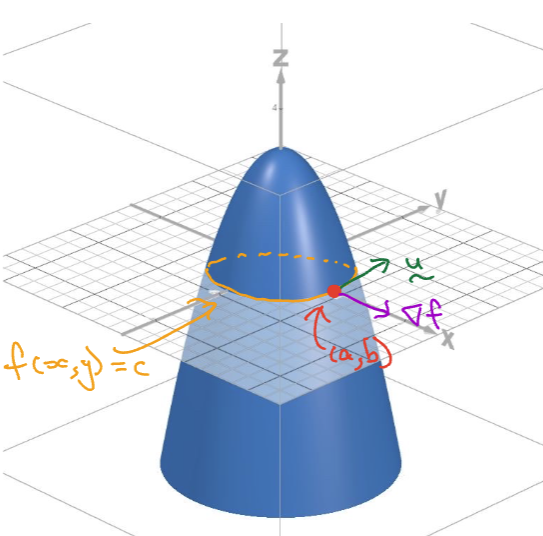
\includegraphics[width=\linewidth]{Graphs/w10_1.png}

    $f(x,y)$ is a constant on the level curve on the $f(x,y)=c$, so the directional derivative of f at $(a,b)$ in the direction of the tangent vector $\vect{u}$ must be zero. So we have
    $$
      D_{\unitv{u}}f(a,b) = \nabla f(a,b) \unitv{u} = 0
    $$
    Hence, \hl{$\nabla f(a,b)$ is orthogonal to the level curve $f(x,y)=f(a,b)$}

    \item \textbf{Equation of a tangent to a level curve:} Given a differentiable function
    $$
      f: D \rightarrow R, D \subseteq R^2
    $$
    we can find  an equation of the tangent line to a level curve $f(x,y) = c$ at $(a,b)$

    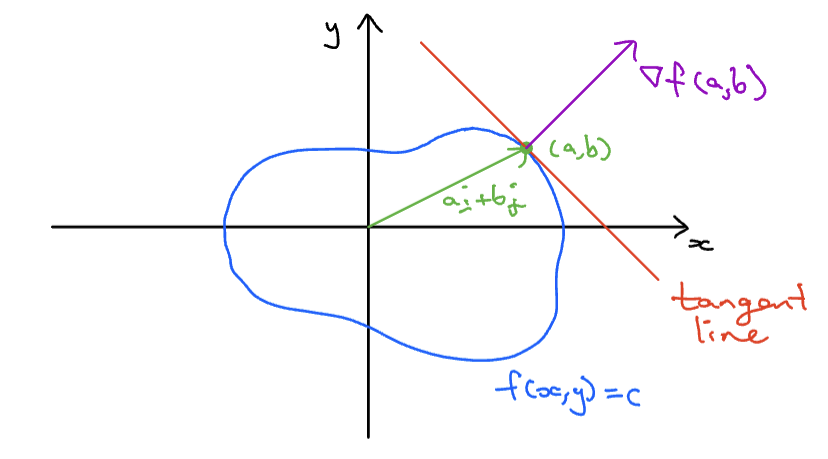
\includegraphics[width=\linewidth]{Graphs/w10_2.png}

    \begin{itemize}
      \item The tangent line has \hl{normal form}:
      $$
        \nabla f(a,b) ((x-a)\vect{i} + (y-b)\vect{j}) = 0
      $$

      \item general form:
      $$
        f_x(a,b)(x-a) + f_y(a,b)(y-b) = 0
      $$
    \end{itemize}

    \item \hl{\textbf{property}}\\\\

    Recall that:
    $$
      D_{\vect{u}}f = \nabla f \unitv{u} = \len{\nabla f} \cos{\theta}
    $$
    Thus, we have
    $$
      -\len{\nabla f} \leq D_{\vect{u}}f \leq \len{\nabla f}
    $$
    \begin{itemize}
      \item The maximum value  $D_{\vect{u}}f = \len{\nabla f}$ occurs when
      $$
        \cos{\theta} = 1 \leftrightarrow \theta = 0 \leftrightarrow \vect{u} = k \nabla f 
      $$
      $\vect{u} = k \nabla f \rightarrow$ \hl{same direction}

      \item The minimum value  $D_{\vect{u}}f = -\len{\nabla f}$ occurs when
      $$
        \cos{\theta} = -1 \leftrightarrow \theta = \pi \leftrightarrow \vect{u} = -k \nabla f 
      $$
      $\vect{u} = -k \nabla f \rightarrow$ \hl{opposite direction}
    \end{itemize}

    Now, suppose $\vect{u} = u_i\vect{i} + u_2\vect{j}$ is tangent to the level curve $f(x,y)=c$

    Since $f$ is constant on the level curve, the directional derivative in the direction of $\vect{u}$ must be zero:
    $$
      D_{\vect{u}}f = \nabla f \vect{u} = u_1 f_x + u_2 f_y = 0
    $$

    So \hl{$\nabla f = f_x \vect{i} + f_y \vect{j}$} is orthogonal to $\vect{u}$, and we can take $u_1 = -f_y$,$u_2 = f_x$, so

    $$
      \vect{u} = - f_y \vect{i} + f_x \vect{j}
    $$
    is tangent to the level curve.

    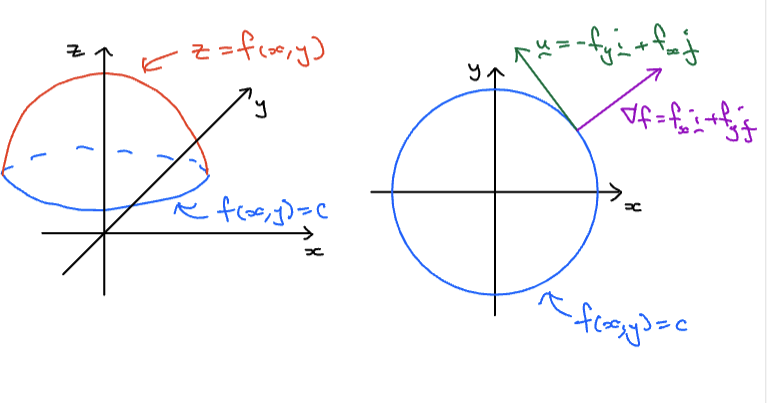
\includegraphics[width=\linewidth]{Graphs/w10_6.png}

  \end{itemize}

  \subsection*{Critical Points}
    \begin{itemize}
      \item A \hl{critical point} of a differentiable function $f: D \rightarrow, D \subseteq R^2$ is a point $(a,b) \in D$ such that:
      $$
        \nabla f(a,b) = \vect{0}
      $$

      \item Types of Critical Points

      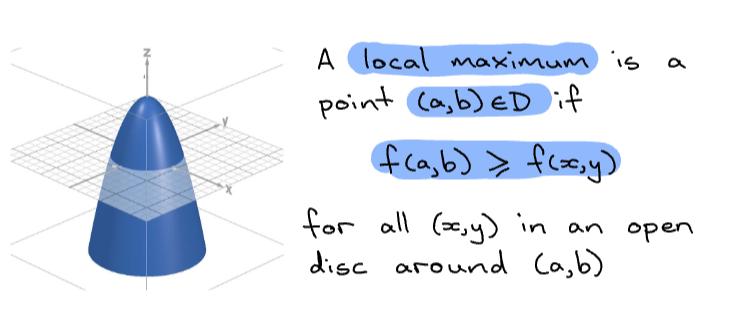
\includegraphics[width=\linewidth]{Graphs/w10_3.png}

      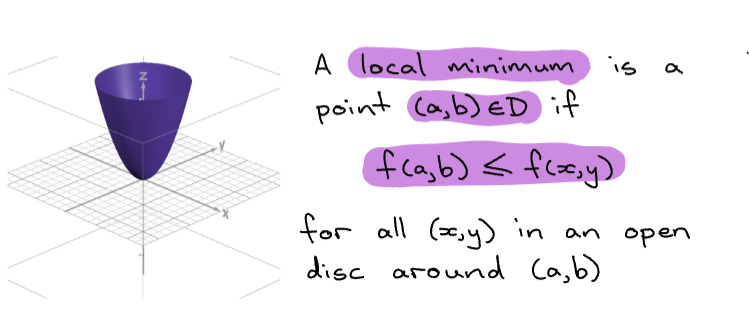
\includegraphics[width=\linewidth]{Graphs/w10_4.png}

      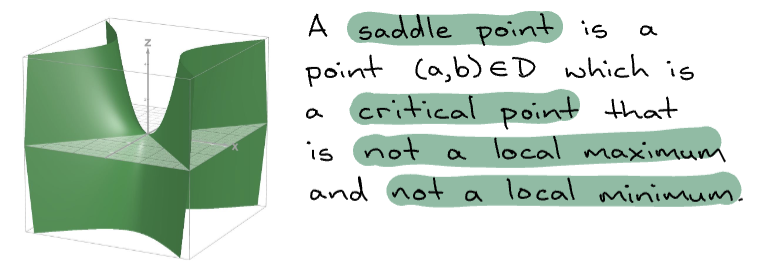
\includegraphics[width=\linewidth]{Graphs/w10_7.png}

      \item \hl{\textbf{discriminant}}: The dicriminant of a differentiable function $f: S \rightarrow R, S \subseteq R^2$ with differentiable first-order partial derivatives is 
      $$
        D(x,y) =f_{xx}(x,y)f_{yy}(x,y) - f_{xy}(x,y)^2
      $$

      \item \textbf{Sceond derivative test}: Let $f: S \rightarrow R, S \subseteq R^2$ be a differentiable function, and $(a,b) \in S$ a critical point of f. Then:
      \begin{itemize}
        \item $D(a,b)<0 \implies  (a,b)$ is a saddle point
        \item $D(a,b) > 0,f_{xx}(a,b)<0 \implies (a,b)$ is a local maximum
        \item $D(a,b) > 0,f_{xx}(a,b)>0 \implies (a,b)$ is a local minimum
      \end{itemize}
    \end{itemize}

  \subsection*{High Order partial derivavtives}
  \begin{itemize}
    \item Suppose we haves a differentiable function:
    $$
     f: D \rightarrow R, D \subseteq R^2
    $$
    with first-order partial derivatives. We define:

    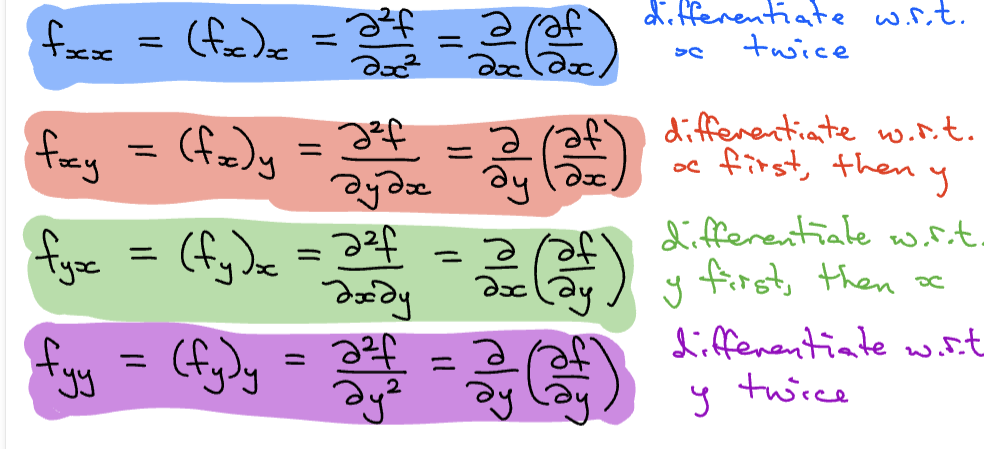
\includegraphics[width=\linewidth]{Graphs/w10_5.png}

    \item \textbf{Theorem:} If $f$ has continuouts partial derivatives near $(a,b)$ then
    $$
      f_{xy}(a,b) = f_{yx}(a,b)
    $$
  \end{itemize}

  \section*{week 12}
  \subsection*{Global Extrema}
  \begin{itemize}
    \item \textbf{Definition:} Lef $f:S \rightarrow R, s \subseteq R^2$ be a function of 2 variables. 
    \begin{itemize}
      \item A point $(a,b) \in S$ is a \hl{global maximum} of $f$
      $$
        f(a,b) \geq f(x,y)
      $$ 
      for all $(x,y) \in S$

      \item A point $(a,b) \in S$ is a \hl{global minimum} of $f$
      $$
        f(a,b) \leq f(x,y)
      $$ 
      for all $(x,y) \in S$
    \end{itemize}

    \item \textbf{When can global extrema occur}
    \begin{itemize}
      \item A set $S \subseteq R^2$ is \hl{closed} if it contains all points in its boundary
      \item A set $S \subseteq R^2$ is \hl{bounded} if it is contained in a sufficiently large disc
    \end{itemize}

    \item \textbf{Fact:} If $f: S \rightarrow R, S \subseteq R^2$ is continuous, and S is closed and bounded, then f attains a global maximum and global minimum on S.

    \item \textbf{Method for finding global extrema:} If \( f: S \to \mathbb{R} \) is differentiable (hence continuous) and \( S \subset \mathbb{R}^2 \) is closed and bounded, then we can find the global extrema on \( S \) by:

    \begin{enumerate}
        \item Finding all critical points of \( f \) on \( S \) by solving \( \nabla f = 0 \).
        
        \item Parameterizing the boundary of \( S \) by \( x(t), y(t) \), \( t \in [a, b] \), and finding any critical points of \( f \) restricted to the boundary of \( S \) by solving \( g'(t) = 0 \) for \( g(t) = f(x(t), y(t)) \).
        
        \item Finding any endpoints of the boundary.
        
        \item Comparing function values at all points found above.
    \end{enumerate}

  \end{itemize}



\end{document}

